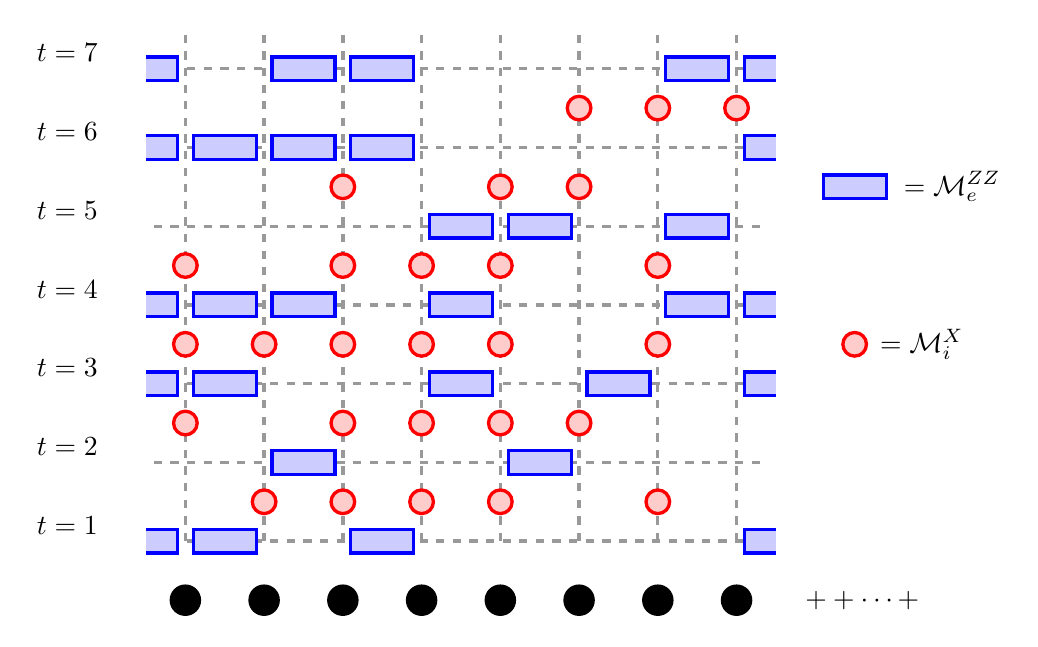
\begin{tikzpicture}

% Define grid dimensions, 10x8 grid
\def\qubits{7} 
\def\timesteps{6}

% Draw the background grid
\foreach \x in {0,...,\qubits} {
  \draw[gray!80, dashed, very thick] (\x,0) -- (\x,\timesteps+.5);
  \fill[black] (\x,-.75) circle (.2);
}
\foreach \t in {0,...,\timesteps} {
  \draw[gray!80, dashed, very thick] (-.4,\t) -- (\qubits+.4,\t);
}

%\draw[red, very thick, fill=red!20] (0,\timesteps+1.2) circle (.15);
%\draw[arrow, thick] (-1,-1) -- (-1,\timesteps+1) node[anchor=west] {\LARGE$t$}; 
\foreach \t in {1,...,\qubits} {
  \node[] at (-1.5,\t-.8) {$t=\t$};
}

% ZZ Measurements with probability p=0.5 on the edges of the grid
\foreach \x in {0,...,\qubits}
    \foreach \t in {0,...,\timesteps} {
        \pgfmathrandominteger{\randnum}{0}{1}
        \ifnum\randnum=1
          % Periodic boundary conditions. Qubits on the right get wrapped around
            \ifnum\x=\qubits
                % Right half
                \fill[blue!20] (\qubits+0.1,\t-0.15) rectangle (\qubits+0.5,\t+0.15);
                \draw[blue,very thick] (\qubits+0.1,\t-0.15) -- (\qubits+0.1,\t+0.15);  % Right border 
                \draw[blue,very thick] (\qubits+0.083,\t-0.15) -- (\qubits+0.5,\t-0.15);      % bottom border
                \draw[blue,very thick] (\qubits+0.083,\t+0.15) -- (\qubits+0.5,\t+0.15);      % top border
                
                % Left half - no border on right side
                \fill[blue!20] (-0.5,\t-0.15) rectangle (-0.1,\t+0.15);
                \draw[blue,very thick] (-0.1,\t-0.15) -- (-0.1,\t+0.15);                % left border
                \draw[blue,very thick] (-0.5,\t-0.15) -- (-0.083,\t-0.15);                   % bottom border
                \draw[blue,very thick] (-0.5,\t+0.15) -- (-0.083,\t+0.15);                   % top border
              \else
                % Normal rectangle for non-boundary positions
                \draw[blue,very thick, fill=blue!20] (\x+0.1,\t-0.15) rectangle (\x+0.9,\t+0.15);
            \fi
            %\draw[blue, fill=blue!30] (\x+0.1,\t-0.15) rectangle (\x+0.9,\t+0.15);
        \fi
    }

\def\loopend{5}
% Place red circles on vertical edges with 0.5 probability
\foreach \x in {0,...,\qubits} {
    \foreach \t in {0,...,\loopend} {
        \pgfmathrandominteger{\randnum}{0}{1}
        \ifnum\randnum=1
            \draw[red, very thick, fill=red!20] (\x,\t+0.5) circle (0.15);
        \fi
    }
  }

  \draw[blue, very thick, fill=blue!20] (\qubits+1.1,4.35) rectangle
  (\qubits+1.9, 4.65);
  \node[anchor=west] at (\qubits+2,4.5) {$=\mathcal{M}^{ZZ}_e$};

  \draw[red, very thick, fill=red!20] (\qubits+1.5,2.5) circle (.15);
  \node[anchor=west] at (\qubits+1.7,2.5) {$=\mathcal{M}^X_i$};

  \node[anchor=west] at (\qubits+.75,-.75) {$\ket{++\cdots+}$};
\end{tikzpicture}
